
\newpage

\section*{Appendix Overview}

% The appendix is organized as follows. Section~\ref{sec:visual} includes additional visual examples illustrating the workflow and effectiveness of the \NAME{} method across the MATH, GPQA, and GSM8K datasets. Section~\ref{supp_sec:std_error} provides a statistical analysis of standard errors to demonstrate the consistency of our experimental results. Section~\ref{sec:randomness} evaluates the robustness of \NAME{} against randomness introduced by varying the temperature settings. Section~\ref{sec:SLM-Mux-vs-majority} analyzes in detail why \NAME{} outperforms majority voting, especially on challenging problems. Section~\ref{sec:single-models} reports the accuracy results for individual models used in our experiments. Section~\ref{sec:licenses} provides the licensing details for the datasets. \cw{TODO update this}

The appendix is organized as follows. Section~\ref{sec:visual} presents additional visual examples illustrating the workflow and effectiveness of the \NAME{} method across the MATH, GPQA, and GSM8K datasets. Section~\ref{sec:slm-failure} provides a detailed analysis of SLM failures in discussion-based orchestration methods, drawing on experiment logs to highlight common failure patterns. Section~\ref{sec:single-models} reports the accuracy of individual models used in our experiments. Finally, Section~\ref{sec:licenses} provides the licensing details for the datasets.


\section{LLM Usage Statement}
\label{sec:usage}

We used Cursor for coding. Large language models (LLMs) were employed to help polish drafts written by humans, and to assist in searching for related papers. The final choice of related work included in this paper was made entirely by the human authors after careful screening. LLMs were also used for proofreading and for providing suggestions.

% \section{LLM Usage Statement}
% \label{sec:visual}


\section{Additional Visual Illustrations of \NAME{}}
\label{sec:visual}

To more effectively illustrate the workflow of our proposed composition method, we select several representative examples from the logs. We demonstrate them in Figure~\ref{fig:example_1}, Figure~\ref{fig:example_2} and Figure~\ref{fig:example_3}.

\paragraph{\NAME{} surpasses majority voting in scenarios with initial disagreement among models.} As illustrated by Figure~\ref{fig:example_1}, during the independent generation phase, Gemma-2-27B is the sole model to provide the correct answer. Hence, majority voting applied directly would fail to select the correct author. 


\begin{figure}[ht]
    \centering
    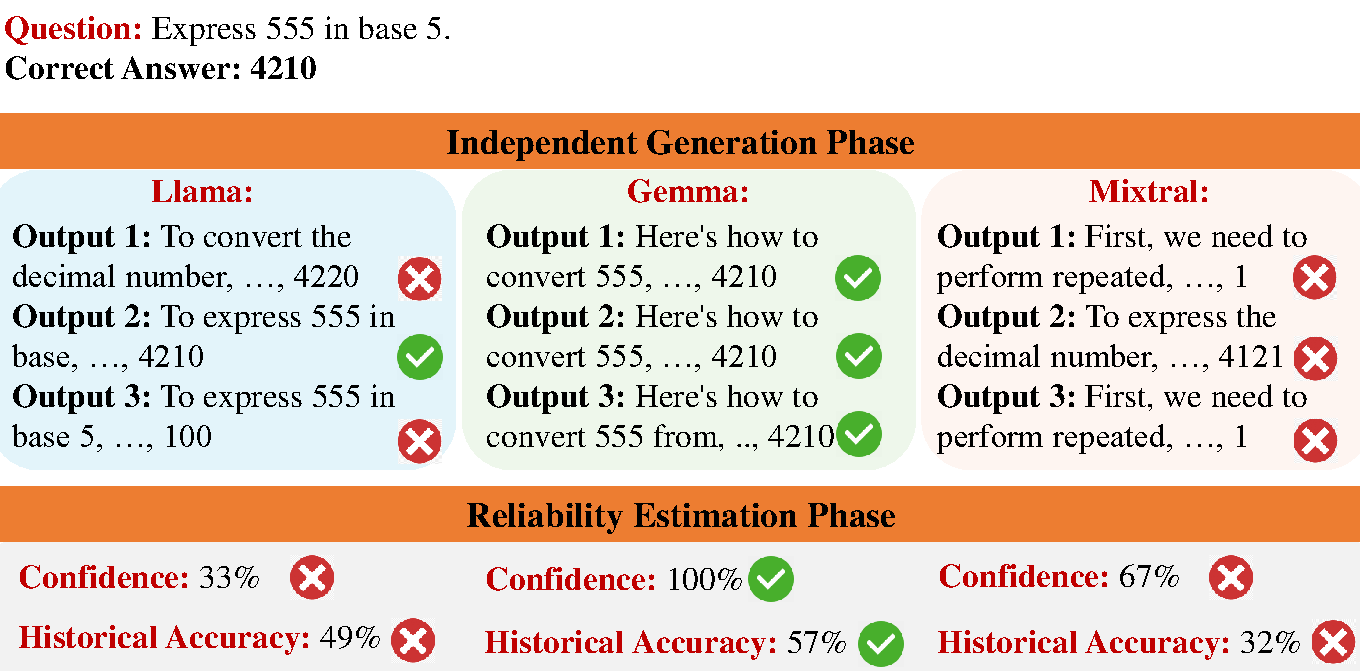
\includegraphics[width=0.7\linewidth]{Figures/example_1_cropped.pdf}
    \caption{\textbf{An illustration of the \NAME{} method applied to the MATH dataset.} In the independent generation phase, three models are used: LLaMA-3.1-8B (denoted as Llama), Gemma-2-27B (denoted as Gemma), and Mixtral-8$\times$7B (denoted as Mixtral). Because the three models provide different answers at first, so each model is invoked two more times. Gemma obtains the highest confidence score and is therefore selected as the final output.}
    \label{fig:example_1}
\end{figure}

\begin{figure}[ht]
    \centering
    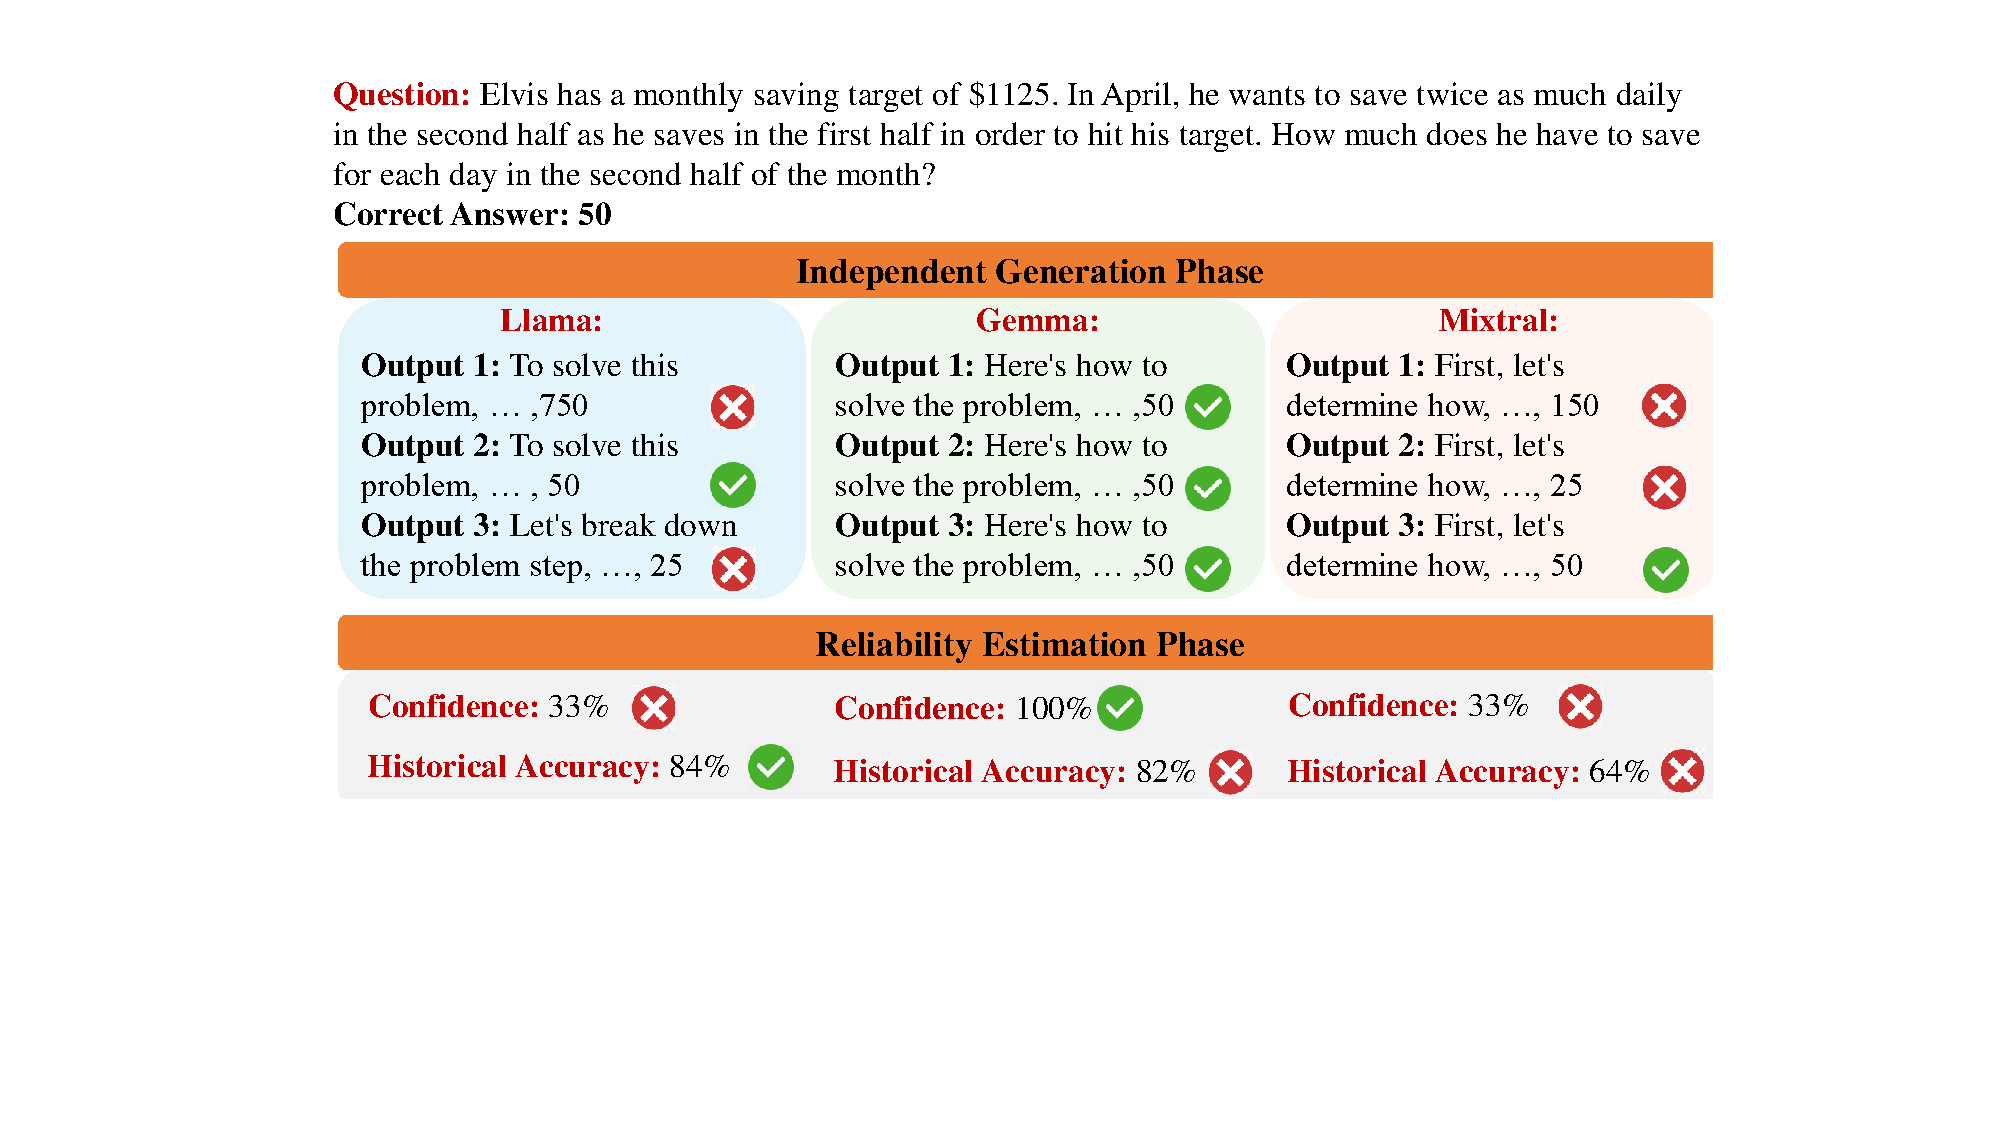
\includegraphics[width=0.7\linewidth]{Figures/example_2_cropped.pdf}
    \caption{\textbf{An illustration of the \NAME{} method applied to the GSM8K dataset.} In the independent generation phase, different models produce different answers. However, when we invoke each model multiple times, we observe that Llama and Mixtral only yield correct answers approximately one-third of the time. In contrast, Gemma demonstrates stable performance.}
    \label{fig:example_2}
\end{figure}

\begin{figure}[ht]
    \centering
    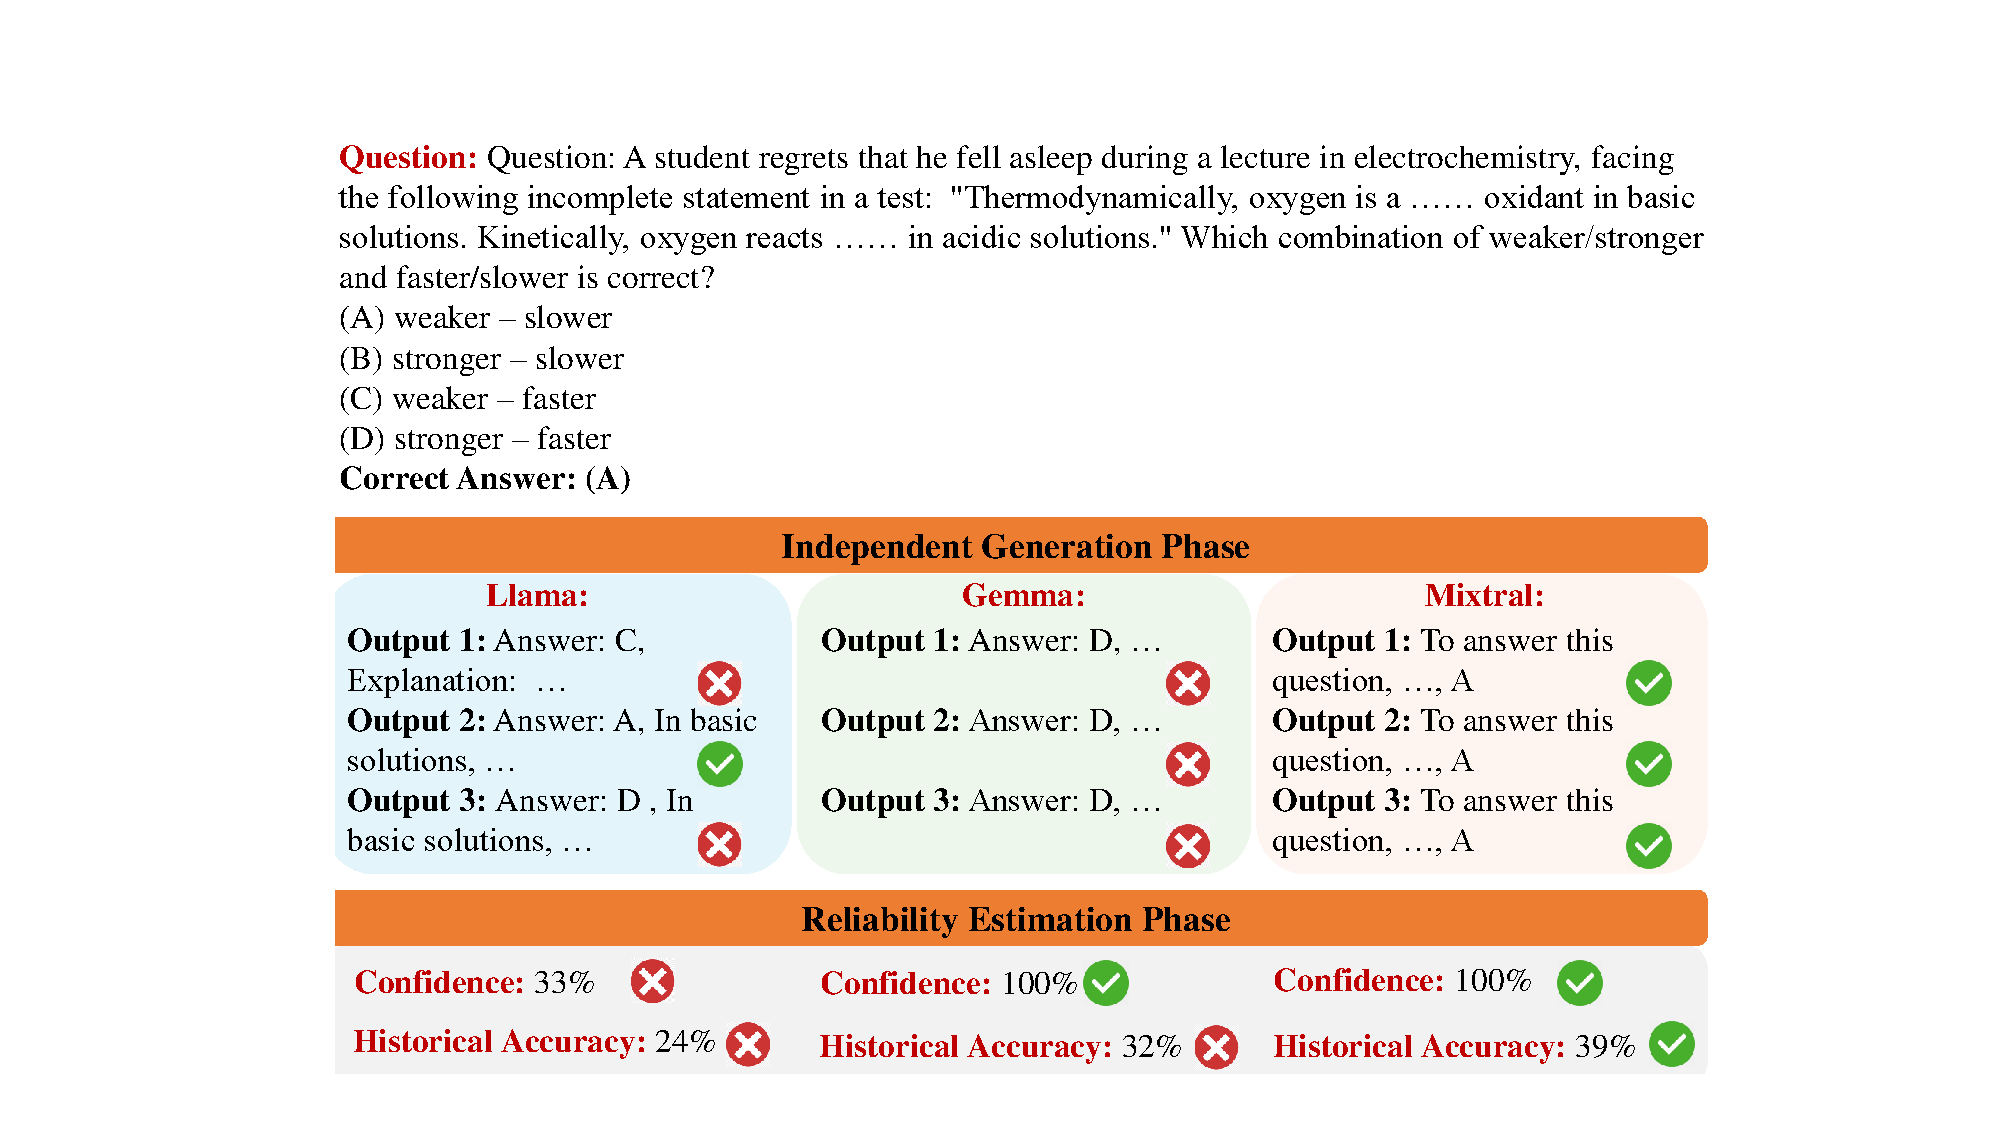
\includegraphics[width=0.7\linewidth]{Figures/example_3_cropped.pdf}
    \caption{\textbf{An illustration of the \NAME{} method applied to the GPQA dataset.} During the independent generation phase, Gemma and Mixtral obtain the same confidence score. However, considering historical accuracy, Mixtral ranks higher. Therefore, Mixtral's answer is selected as the final output.}
    \label{fig:example_3}
\end{figure}



% \section{Analyzing Standard Error in Results}
% \label{supp_sec:std_error}
% To support our primary claim that the proposed method yields a significant improvement in accuracy (as shown in Table~\ref{tab:composition-combined}), we further analyze the statistical significance in our experimental results. Specifically, we analyze logs from experiments and compute the standard error (standard deviation divided by the square root of the number of samples) across different samples. The results of this analysis are presented in Table~\ref{tab:SLM-Mux-results-se}. We observe that the standard error associated with our method is relatively small, indicating consistency and reliability in benchmark performance. 

% To quantify the uncertainty associated with our reported accuracies, we computed the standard error by treating the correctness of each response as an independent Bernoulli random variable. Specifically, for each item, we assign a binary value \( X_i \), where \( X_i = 1 \) indicates a correct response and \( X_i = 0 \) an incorrect one. Given an empirical accuracy \(\hat{p} = \frac{1}{n}\sum_{i=1}^{n} X_i\) computed over \(n\) samples, the standard error (SE) of this accuracy estimate is calculated as follows:

% \[
% \text{SE} = \sqrt{\frac{\hat{p}(1 - \hat{p})}{n}}.
% \]

% This standard error serves as the basis for the error bars presented in Table~\ref{tab:SLM-Mux-results-se}, reflecting the expected magnitude of sampling variability if the experiment were repeated under identical conditions.

% \begin{table}[ht]
% \centering
% \small
% \begin{tabular}{lccc}
% \toprule
% \textbf{Method} & \textbf{MATH Acc (\%)} & \textbf{GPQA Acc (\%)} & \textbf{GSM8K Acc (\%)} \\
% \midrule
% Mixture-of-Agents          & 51.4 $\pm$ 2.24 & 33.3 $\pm$ 3.37 & 81.6 $\pm$ 1.73 \\
% LLM-Debate                  & 51.6 $\pm$ 2.23 & 36.8 $\pm$ 3.44 & 80.8 $\pm$ 1.76 \\
% Multi-Agent Verification    & 48.4 $\pm$ 2.23 & 35.3 $\pm$ 3.41 & 86.4 $\pm$ 1.53 \\
% \textbf{\NAME{} (Ours)}         & \textbf{63.0 $\pm$ 2.16} & 41.9 $\pm$ 3.52 & \textbf{88.4 $\pm$ 1.43} \\
% \midrule
% Single-Best                 & 56.8 $\pm$ 2.22 & 38.9 $\pm$ 3.48 & 84.2 $\pm$ 1.63 \\
% Single-Best-SC              & 58.0 $\pm$ 2.21 & \textbf{42.4 $\pm$ 3.53} & 86.8 $\pm$ 1.51 \\
% Upper Bound                 & 64.6 $\pm$ 2.14 & 57.0 $\pm$ 3.54 & 92.0 $\pm$ 1.21 \\
% \bottomrule
% \end{tabular}
% % \vspace{5pt}
% \caption{\small \textbf{Accuracy with Standard Error.} The standard error across MATH, GPQA, and GSM8K for various methods. \NAME{} demonstrates relatively small standard errors.}
% \label{tab:SLM-Mux-results-se}
% % \vspace{-5pt}
% \end{table}


% \section{Analyzing Randomness in Results}
% \label{sec:randomness}
% Given that our method incorporates stochasticity solely through temperature settings greater than zero, we conducted additional experiments to explicitly quantify the randomness introduced by varying temperature values. The results, summarized in Table~\ref{tab:SLM-Mux-results-temp}, demonstrate that our approach exhibits strong robustness with respect to temperature-induced variability.

% \begin{table}[htbp]
% \centering
% \small
% \begin{tabular}{lccc}
% \toprule
% \textbf{Method} & \textbf{MATH Acc (\%)} & \textbf{GPQA Acc (\%)} & \textbf{GSM8K Acc (\%)} \\
% \midrule
% \textbf{\NAME{} (Ours)} & 61.8 $\pm$ 1.2 & 42.1 $\pm$ 0.3 & 87.8 $\pm$ 0.6 \\
% \bottomrule
% \end{tabular}
% \vspace{5pt}
% \caption{\small \textbf{Accuracy with Temperature-error bars of \NAME{} Method.}}
% \label{tab:SLM-Mux-results-temp}
% \end{table}




% \section{Analysis on Why \NAME{} Outperforms Majority Voting Methods like Agent Forest}
% \label{sec:SLM-Mux-vs-majority}

% Majority voting only improves accuracy for simpler tasks. Our experimental results indicate that majority voting enhances accuracy solely when applied to simple questions, and it does not outperform the best individual LLM prediction for complex problems. Through detailed analysis, we observed that for simpler questions, disagreements among individual LLM predictions are typically limited, whereas for complex problems, such disagreements become significantly pronounced. We model this problem by assuming each LLM independently generates answers, where each answer has a probability \( p \) of being correct. Under this assumption, the theoretical accuracy \( A(N, p) \) achievable by majority voting among \( N \) independently predicting models is described by the cumulative probability of a binomial distribution:

% \begin{equation}
% A(N, p) = \Pr\left(X \ge \left\lceil \frac{N}{2} \right\rceil\right) = \sum_{k=\lceil \frac{N}{2} \rceil}^{N} \binom{N}{k} p^{k}(1 - p)^{N - k}, \quad X \sim \text{Binomial}(N, p)
% \end{equation}

% % Placeholder for composed accuracy figure
% \begin{figure}[ht]
%     \centering
%     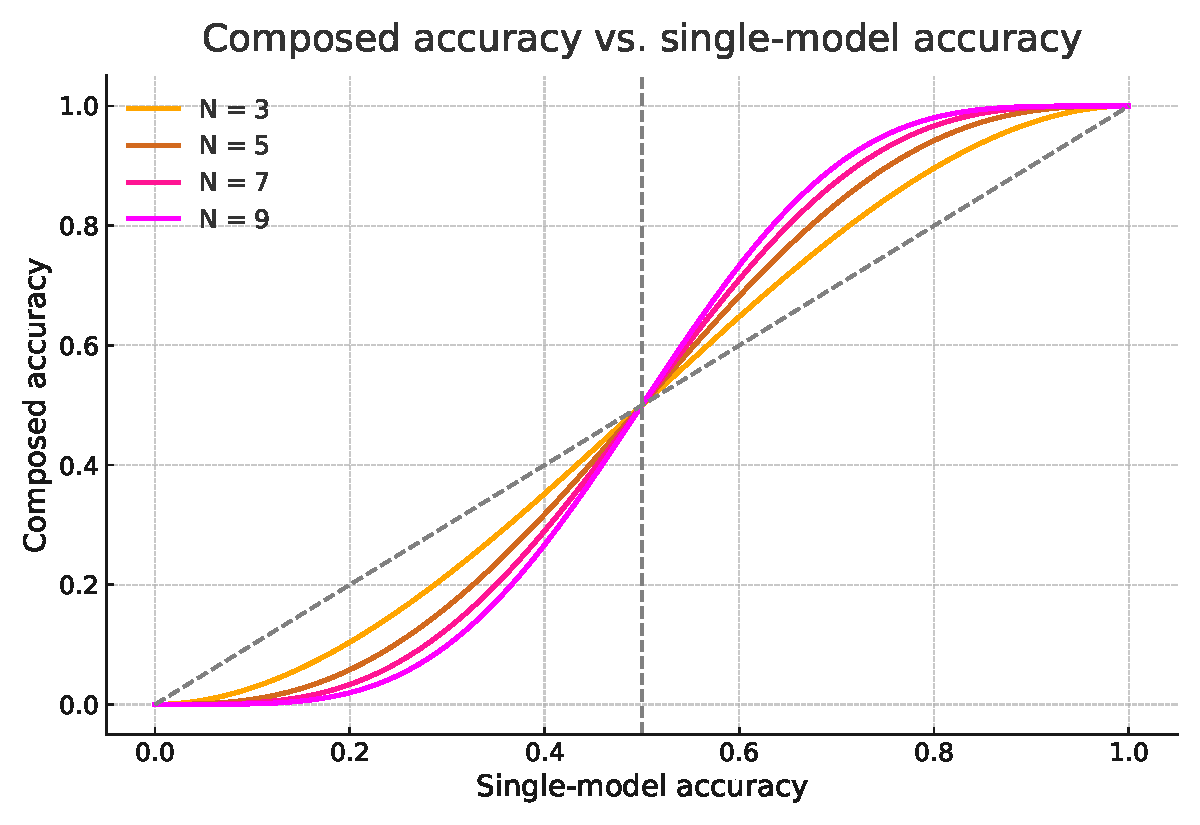
\includegraphics[width=0.7\linewidth]{Figures/composed_accuracy.pdf}
%     \caption{\textbf{Compared with Composed Accuracy and Single-model Accuracy.} Theoretical composed accuracy $A(N, p)$ as a function of individual accuracy $p$ for different numbers of models ($N = 3, 5, 7, 9$).}
%     \label{fig:composed_accuracy}
% \end{figure}

% In Figure~\ref{fig:composed_accuracy}, we plot the theoretical accuracy \( A(N, p) \) as a function of individual accuracy \( p \) for different numbers of models (\( N = 3, 5, 7, 9 \)). This plot clearly demonstrates that composed accuracy \( A(N, p) \) surpasses individual accuracy \( p \) only when \( p > 0.5 \). Conversely, for values of \( p \leq 0.5 \), majority voting negatively impacts performance, indicating that aggregation is counterproductive when individual models perform near or below chance.

% When multiple LLMs with varying accuracies participate in a simple majority vote, those with lower accuracy (close to or below chance level, i.e., $\leq 0.5$) can substantially dilute the contribution of higher-performing models. Essentially, the errors made by lower-accuracy models may dominate the voting outcome, pulling down the overall accuracy rather than enhancing it.

% In contrast, \NAME{} addresses this limitation by first evaluating each model’s consistency and confidence internally through multiple self-sampled predictions. Models that fail to demonstrate consistent confidence in their answers are filtered out, ensuring only the predictions from reliable, higher-performing models contribute significantly to the final decision. Furthermore, \NAME{} employs historical accuracy records of each model as prior knowledge to weight decisions effectively, further enhancing its ability to select the optimal predictions.

% Thus, while majority voting indiscriminately aggregates predictions, potentially amplifying errors from weaker models, \NAME{} selectively incorporates predictions, significantly improving accuracy, particularly in challenging scenarios.

% \section{Situations in Which \NAME{} is Less Effective}
% \label{{sec:SLM-Mux-less-effective}}


\section{Detailed Analysis of SLM Failures in Discussion-Based Methods}
\label{sec:slm-failure}

% We analyze the experiment logs of LLM-Debate when using SLMs, specifically the one presented in Section~\ref{sec:comparison}.
% This file contains 242 failure debate logs out of 500. We first prompt another analyzer LLM to analyze the reason for the failure; after we get the 242 analyses generated by the analyzer LLM, we then prompted another LLM, we then prompted another LLM to label the logs whterh they are failed due to groupthinking. We get 16? of our 242 labeled as yes. Which reinforce our statement. 

% The prompt in the analyzor LLMs and labelor aredemonstrated in box below


We analyze the experiment logs of LLM-Debate using small language models (SLMs) in Section~\ref{sec:comparison}. Among 500 debate problems, 242 resulted in failure (48.4\%). For each of the 242 failed debates, we first used an analyzer LLM to produce a process-focused failure analysis. We then used a separate labeling LLM to classify whether each failed debate was due to groupthink.


The labeling results are shown in Table~\ref{tab:label}:

\begin{table}[t]
\centering
\begin{tabular}{@{}l r l@{}}
\toprule
Metric & Count & Rate \\
\midrule
Total Debates Analyzed & 500 & 100\% of total \\
Failed Debates (System Error) & 242 & 48.4\% of total \\
\midrule
\multicolumn{3}{@{}l}{\textit{Breakdown of Failed Debates:}} \\
\quad Attributed to Groupthink & 144 & 59.5\% of failures \\
\quad Attributed to Other Causes & 79 & 32.6\% of failures \\
\quad Classification Unsuccessful & 19 & 7.9\% of failures \\
\bottomrule
\end{tabular}
\caption{\textbf{Failure Cause Attribution} This table shows the cause attribution for LLM-Debate when involving SLMs.}
\label{tab:label}
\end{table}

These results reinforce our claim that groupthink is a major failure mode in SLM-based LLM-debate.

We provide the exact prompts used by (i) the analyzer LLM to generate the 242 failure analyses (Figure~\ref{lst:prompt-analyzer}) and (ii) the groupthink labeler LLM to classify groupthink (Figure~\ref{lst:prompt-groupthink-system}). Placeholders such as \texttt{\{problem\}} indicate runtime substitutions by our code.

% \noindent Source: \texttt{analyze\_incorrect\_problems.py} (function \texttt{create\_analysis\_prompt})
% (previous content above lstlisting)
\lstdefinestyle{promptstyle}{basicstyle=\ttfamily,breaklines=true,backgroundcolor=\color{gray!10}}

% \begin{minipage}{\linewidth}
% \begin{lstlisting}[style=promptstyle][style=promptstyle]
% As an expert in analyzing multi-agent AI systems, your task is to analyze why an 'LLM Debate' process failed to find the correct answer. Your focus should be on the *debate dynamics and process*, not just the mathematical details. The goal is to understand the failure of the debate methodology itself.

% **Ground Truth:**
% - **Problem Statement:** {problem}
% - **Correct Answer:** {ref_answer}

% **Debate Information:**
% - **Final Incorrect Answer from System:** {system_answer}

% **Analysis of Round 1:**
% - **Model `{model_name}` proposed:**
%   - Answer: `{extracted_answer}`
%   - Reasoning:
% ```
% {full_text}
% ```

% ... (repeats per round and per model)

% **Your Analysis Task:**
% Based on the debate history, provide a "Debate Failure Analysis". Do not focus on simple calculation mistakes. Instead, analyze the interaction between the models and the structure of the debate. Pinpoint the core reasons the *debate process* failed. Consider these questions:

% 1.  **Error Propagation vs. Correction:** How did initial errors influence later rounds? Were there moments where a correct idea was introduced but ignored or overruled? Why did the debate fail to self-correct?
% 2.  **Groupthink and Influence Dynamics:** Did the models converge on a flawed consensus? Did one or more influential but incorrect models lead the group astray? Was there evidence of independent reasoning that was shut down?
% 3.  **Argumentation Quality:** Did the models provide convincing but ultimately flawed arguments? Did they effectively challenge each other's reasoning, or was the debate superficial?
% 4.  **Critical Failure Point in the Debate:** Identify the single most critical turn or moment in the debate that sealed its failure. What happened, and why was it so impactful?
% 5.  **Improving the Debate:** What is the single most important change to the debate protocol or dynamics that could have prevented this failure? (e.g., different communication rules, promoting dissident opinions, etc.)

% Provide a concise, expert analysis focusing on the *process* failure.
% \end{lstlisting}
% \caption{Analyzer Prompt}
% \end{minipage}


\begin{figure}[htbp]
  \begin{minipage}{\linewidth}
  \begin{lstlisting}[style=promptstyle]
As an expert in analyzing multi-agent AI systems, your task is to analyze why an 'LLM Debate' process failed to find the correct answer. Your focus should be on the *debate dynamics and process*, not just the mathematical details. The goal is to understand the failure of the debate methodology itself.

**Ground Truth:**
- **Problem Statement:** {problem}
- **Correct Answer:** {ref_answer}

**Debate Information:**
- **Final Incorrect Answer from System:** {system_answer}

**Analysis of Round 1:**
- **Model `{model_name}` proposed:**
  - Answer: `{extracted_answer}`
  - Reasoning:
```
{full_text}
```

... (repeats per round and per model)

**Your Analysis Task:**
Based on the debate history, provide a "Debate Failure Analysis". Do not focus on simple calculation mistakes. Instead, analyze the interaction between the models and the structure of the debate. Pinpoint the core reasons the *debate process* failed. Consider these questions:

1.  **Error Propagation vs. Correction:** How did initial errors influence later rounds? Were there moments where a correct idea was introduced but ignored or overruled? Why did the debate fail to self-correct?
2.  **Groupthink and Influence Dynamics:** Did the models converge on a flawed consensus? Did one or more influential but incorrect models lead the group astray? Was there evidence of independent reasoning that was shut down?
3.  **Argumentation Quality:** Did the models provide convincing but ultimately flawed arguments? Did they effectively challenge each other's reasoning, or was the debate superficial?
4.  **Critical Failure Point in the Debate:** Identify the single most critical turn or moment in the debate that sealed its failure. What happened, and why was it so impactful?
5.  **Improving the Debate:** What is the single most important change to the debate protocol or dynamics that could have prevented this failure? (e.g., different communication rules, promoting dissident opinions, etc.)

Provide a concise, expert analysis focusing on the *process* failure.
\end{lstlisting}
  \end{minipage}
  \caption{Prompt Template for Failure Analysis.}
  \label{lst:prompt-analyzer}
\end{figure}

\begin{figure}[htbp]
  \begin{minipage}{\linewidth}
  \begin{lstlisting}[style=promptstyle]
You are an expert analyst of multi-agent LLM debates. Your goal is to determine whether the failure primarily involved groupthink/conformity dynamics. Groupthink indicators include: early flawed consensus, explicit capitulation to a majority, social proofing, adopting peers' answers without critique, abandoning independent reasoning to match others, or reinforcing an incorrect majority despite available dissent. Not-groupthink includes failures due to independent arithmetic/logic errors, argument complexity/veneer effects without convergence, or chaotic divergence with no consensus influence. Return STRICT JSON only, with keys: groupthink (bool), confidence (float 0-1), reasons (string), cues (array of strings).
\end{lstlisting}
  \end{minipage}
  \caption{Prompt for Groupthink Classification.}
  \label{lst:prompt-groupthink-system}
\end{figure}

\section{Accuracy of Single LLMs}
\label{sec:single-models}
We evaluated the accuracy of single model accuracy under the condition of temperature equal to zero. The results are shown in Table~\ref{tab:base-models-combined} and Table~\ref{tab:base-models}.

\begin{table}[hbtp]
\centering
\begin{tabular}{lccc}
\toprule
\textbf{Model} & \textbf{MATH Acc (\%)} & \textbf{GPQA Acc (\%)} & \textbf{GSM Acc (\%)} \\
\midrule
Llama-3.1-8B         & 48.6 & 23.7 & 84.2 \\
Mistral-8$\times$7B  & 31.6 & 31.9 & 63.4 \\
Gemma-2-27B          & 56.8 & 38.8 & 81.6 \\
\bottomrule
\end{tabular}
\vspace{5pt}
\caption{\textbf{Small Model Base Performance.} Base model accuracy on MATH, GPQA, and GSM8K.}
\label{tab:base-models-combined}
\end{table}


\begin{table}[hbtp]
\centering
\begin{tabular}{lcccc}
\toprule
\multirow{2}{*}{\textbf{Model}} & \multicolumn{2}{c}{\textbf{MATH}} & \multicolumn{2}{c}{\textbf{GPQA}} \\
\cmidrule(lr){2-3} \cmidrule(lr){4-5}
& \textbf{Accuracy (\%)} & \textbf{Token Usage} & \textbf{Accuracy (\%)} & \textbf{Token Usage} \\
\midrule
DeepSeek V3       & 87.0  & 419,513   & 55.1  & 173,885 \\
Gemini 2.0 Flash  & 90.4  & 361,737   & 63.6  & 195,576 \\
GPT-4o            & 79.8  & 408,410   & 51.0  & 212,037 \\
\bottomrule
\end{tabular}
\vspace{5pt}
\caption{\textbf{Large Model Base Performance.} Base model performance and token usage on MATH and GPQA datasets. Accuracy is the percentage of correct answers, and token usage reflects total tokens consumed (prompt + response) over the entire dataset for each model.}
\label{tab:base-models}
\vspace{-15pt}
\end{table}


\section{Licenses for Datasets}
\label{sec:licenses}
The MATH dataset is licensed under the MIT License.\\
The GPQA dataset is licensed under the Creative Commons Attribution 4.0 International (CC BY 4.0) License.\\
The GSM8K dataset is licensed under the MIT License.
